\subsection{The Condition Predicate}\label{subsec:the-condition-predicate}

In the following sections, we formally define the semantics of \RL and introduce its language features.
The syntax is pure JSON.
Additionally, we back up each language feature with use cases that lead to their implementation.
These requirements are the result of either conducted expert interviews or research in medical billing documents and catalogs.

\subsection{The Condition Triplet pattern}\label{subsec:the-condition-triplet-pattern}
As described in chapter \ref{ch:aspects-of-rule-based-systems}, a rule-based system requires regular maintenance and rule updates.
This refers not only to the rules in the rule base but also to the framework itself.
During the design of the billing framework, I emphasized extendability by using the pattern illustrated in figure \ref{fig:condition-triplet-pattern}.
\begin{figure}
    \centering
    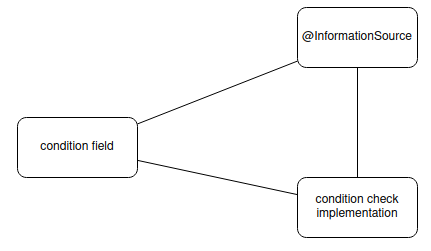
\includegraphics[width=0.75\linewidth]{./figures/condition-triplet-pattern}
    \caption{Generic illustration of the triplet pattern}
    \label{fig:condition-triplet-pattern}
\end{figure}
Adding a new condition type to the condition predicate of \RL requires implementing the condition triplet pattern.

\paragraph{Condition Field}
Each condition type requires a meaningful keyword with a proper data type in the rule language schema.
Generally speaking, complicated condition features tremendously reduce user-friendliness.
Feedback from Dr. Bojko has shown that many simple condition fields are preferable to fewer, more complex ones, as the latter are more prone to errors.
A rule of thumb is to use flag-like boolean-type fields whenever possible.

\paragraph{Information Source}
Each condition subscribes to one or more information sources.
An information source is medical or administrative information that, as part of the research, was identified as relevant for billing.
Each Information source requires a fetch implementation that gets the data from other \AV services and ensures the condition check implementation can access it.

\paragraph{Condition Check Implementation}
Each condition field requires an actual condition implementation that expects a \code{RuleEvaluationInput} object as an input and returns the condition result.
\code{RuleEvaluationInput} objects are data classes that conveniently provide the data that represents fetched information sources required by the existing condition fields.
Section \addref describes them in more detail.

Figure \ref{fig:condition-triplet-pattern-instance-1} and \ref{fig:condition-triplet-pattern-instance-2} illustrate concrete implementations of the condition triplet pattern
for the condition fields \code{newBorn} and \code{minPatientAge}.
Both subscribe to the \code{@InformationSourcePatientAge} information source but have different condition check implementations.

\begin{figure}
    \centering
    \begin{subfigure}[b]{0.45\linewidth}
        \centering
        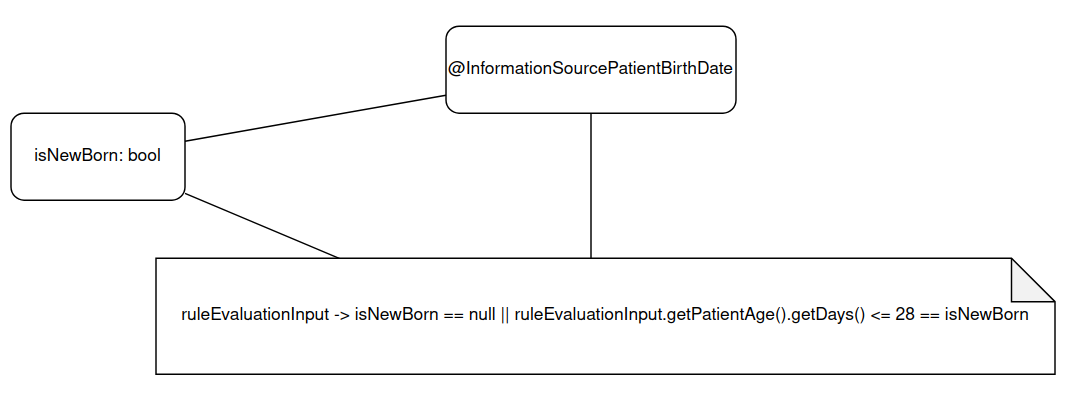
\includegraphics[width=\linewidth]{./figures/ctp-is-new-born}
        \caption{Condition Triplet pattern instance 1}
        \label{fig:condition-triplet-pattern-instance-1}
    \end{subfigure}
    % Adjust or remove the space between figures as needed
    \hspace{5mm} % This adds a bit of horizontal space between the figures
    \begin{subfigure}[b]{0.45\linewidth}
        \centering
        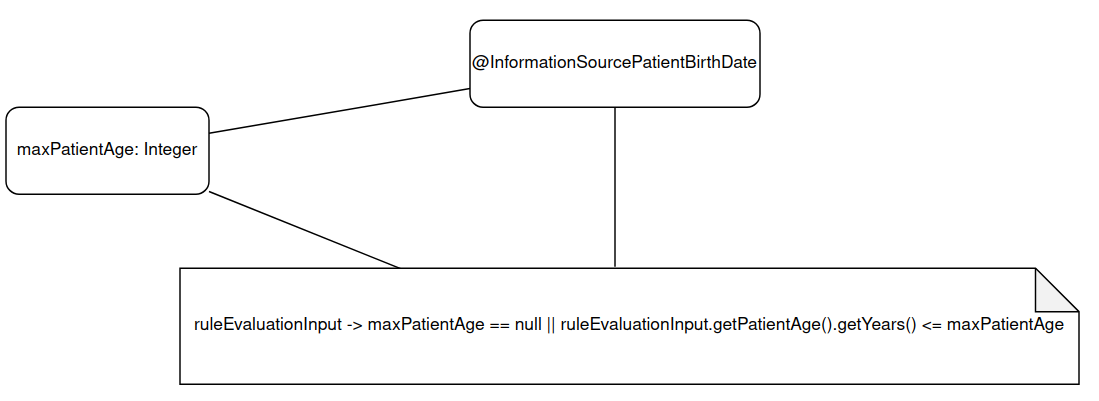
\includegraphics[width=\linewidth]{./figures/ctp-max-patient-age}
        \caption{Condition Triplet pattern instance 2}
        \label{fig:condition-triplet-pattern-instance-2}
    \end{subfigure}
    \label{fig:coffee}
\end{figure}
This section discusses the \code{condition} field of a rule.
Its value is a condition object with the following fields.

\subsection{Patient Related Conditions}\label{subsec:patient-related-conditions}

\paragraph{minPatientAge / maxPatientAge}
\code{minPatientAge} and \code{maxPatientAge} are integer fields that enable restrictions on the patient's age.
Both fields store an integer specifying a number of years.
The user can combine both to require the patient's age to be within a specific age interval.

In medical practice, a patient's age can significantly influence a treatment's complexity.
In cases involving very young or very elderly patients, practitioners may encounter patient age-specific challenges.
Due to these challenges, treatments may require more time, special care, or other additional resources.
As a result, practitioners may apply billing multipliers to compensate for the additional effort.
This is why users can use the \minPatientAge and \maxPatientAge fields to implement these types of multiplier justification rules.
Concrete GOÄ codes such as \goa{K1} and \goa{K2} also require the patient's age.
The patient age is also highly relevant for various EBM codes, but it already exists as a structured condition in the EBM catalog.
This is why using patient age conditions in EBM rules is redundant.
The information source for these two conditions is \code{@InformationSourcePatientAge}


\paragraph{isNewBorn}
\isNewBorn is syntactic sugar and a particular case of the \maxPatientAge condition.
It is a boolean field that denotes whether a patient must be a newborn.
According to the GOÄ, babies at most 28 days old are newborns \cite{bruck1998kommentar}.
It is relevant for \goa{25}, which covers physical examinations for newborns.
It can also be interesting for multiplier justifications.
The information source for these two conditions is \code{@InformationSourcePatientAge}.

\paragraph{patientSpeaksGerman/patientSpeaksEnglish}
\patientSpeaksGerman and \patientSpeaksEnglish are both boolean fields that denote whether the patients can communicate in the respective language.
Communication problems can increase the effort and time a treatment may require and can be justifications for multipliers
\patientSpeaksGerman and \patientSpeaksEnglish subscribe to \code{@InformationSourcePatientLanguages}.

\paragraph{gender}
The \gender condition is an important condition type relevant for various EBM and GOÄ codes.
Its values can either be \code{\"male\"}, \code{\"female\"} or \code{\"diverse\"}
As mentioned in paragraph \ref{par:administrative-gender}, structured EBM records already cover gender conditions, making the \gender condition obsolete for EBM.
It can nonetheless be helpful for gender-specific services such as  \goa{27}, \goa{28},  GOÄ codes in section \mete{H}, Obstetrics and Gynecology, and GOÄ codes in \mete{Urology}.
\gender subscribes to the \code{@InformationSourcePatientGender}.
\paragraph{isPregnant}
The \isPregnant boolean condition is syntactic sugar for a special case of the \anamnesisBlocks condition field.
The following rules are equivalent.
\lstinputlisting[
    language=json,
    style=json,
    caption={\code{isPregnant} rule},
    label={lst:is-pregnant}
]{code/rules/specification/isPregnant.json}
Pregnancy can be a reason for additionally required care or services during a treatment that is not necessarily related to the patient's pregnancy,
making it also a possible justification for multipliers.
It is helpful for codes such as \goa{23}, which applies to initial pregnancy-related examinations.
\code{isPregnant} subscribes to the information source \code{@InformationSourceAnamnesisBlocks}.

\paragraph{isSober}
The \isSober boolean condition describes the patient's current state during the treatment.
A patient is non-sober when under the influence of alcohol or addictive substances.
\isSober is effectively syntactic sugar for a special case of the \anamnesisBlocks condition.
\lstinputlisting[
    language=json,
    style=json,
    caption={\code{is sober} rule},
    label={lst:is-sober}
]{code/rules/specification/isSober.json}


\paragraph{minNumberOfAllergies}
\minNumberOfAllergies is a field that specifies the minimal number of allergies a patient requires.
From medical experts at \AV I have learned that a high number of allergies can make treatments more challenging for several reasons:
\begin{itemize}
    \item It may reduce the number of medical options as medications contain allergens or can produce them in specific environments.
    \item It can increase the complexity of the diagnostic process, as allergy reactions can mimic symptoms of other diagnoses.
    \item Patients with a high number of allergies require increased caution and care.
    Practitioners need to spend more time for history review and patient monitoring.
\end{itemize}
This makes \minNumberOfAllergies a helpful condition for multiplier justifications.
It subscribes to the information source \code{@InformationSourcePatientAllergies}

\subsubsection{Block Content Related Sub-Rules}
A medical treatment consists of multiple stages of patient care.
Each stage has its specific aims and tools.
Anamnesis,
physical examination and procedures represent different stages of patient care and are highly relevant for billing.

\paragraph{Block Content Conditions}\label{par:block-content-field-types}
A proto block content can contain information of different input types.
The billing framework handles and validates each input type differently.

\lstinputlisting[
    language=json,
    style=json,
    caption={\code{minDuration} and \code{maxDuration}},
    label={lst:simple-field-rules}
]{code/rules/specification/blockcontentrules/simple-field-rule.json}

Listing \ref{lst:simple-field-rules} gives an overview how basic block content conditions.
We access physical block contents using the \code{physicalBlock} condition field.
A rule matches if its condition evaluates to true.
Rule 1 matches if a liver palpation is part of the treatment, which is the case if we \code{liverPalpation} block is the set of physical blocks.
Rule 2 matches if a liver palpation is part of the treatment and \code{isLiverPalpable} is set to \true.
Rule 3 is similar to Rule 2 with the difference that \code{liverTexture} is a enumeration field.
Rule 4 specifies multiple field conditions, conjugating all conditions in the block.
We can use the \code{|} operator to disjunct enum values as shown in the \code{liverTexture} field.

Proto contents can have nested sub-object fields.
Listing \ref{lst:nested-object-field-rules} illustrates how we enforce conditions on fields inside nested objects.
\lstinputlisting[
    language=json,
    style=json,
    caption={\code{minDuration} and \code{maxDuration}},
    label={lst:nested-object-field-rules}
]{code/rules/specification/blockcontentrules/nested-object-field-rule.json}

Proto content rules can also have fields where the type is a list of objects.
Rule 5 in listing \ref{lst:object-list-field-rules} matches if a hernia block exists in the treatment and the hernia block has two hernia objects where one is palpable and one is not visible.
\lstinputlisting[
    language=json,
    style=json,
    caption={\code{minDuration} and \code{maxDuration}},
    label={lst:object-list-field-rules}
]{code/rules/specification/blockcontentrules/object-list-field-rule.json}

The previous rules used the \code{physicalBlocks} condition field, which subscribes to \code{@InformationSourcePhysicalBlocks}.
We can use \code{anamnesisBlocks} and \code{procedureBlocks} to apply equivalent conditions on anamesis and procedure blocks.
Both subscribe to \code{@InformationSourceAnamnesisBlocks} and \code{@InformationSourcePhysicalBlocks}, respectively.

\paragraph{Logical expression trees for block contents}\label{par:logical-trees}
Some billing rules depend on more than one block content.
In such cases, we can make use of logical expression trees.
Rule 6 in listing \ref{lst:block-combination-rules} matches if we have a \code{skinChangeExaminations} block with \code{skinChangePresent} set to \true,
a \code{pupilsAndLightReaction} block and a \code{liverpalpation} or a \code{hernias} block in the treatment object.
The system evaluates logical expression trees in a recursive manner starting from the root.
It evaluates inner nodes by evaluating its children and combining their results with their operator.
\lstinputlisting[
    language=json,
    style=json,
    caption={Logical block content tree},
    label={lst:block-combination-rules}
]{code/rules/specification/blockcontentrules/block-combination-rule.json}

\paragraph{minAmountPhysicalBlocks / maxAmountPhysicalBlocks / minAmountAnamnesisBlocks / maxAmountAnamnesisBlocks}
Using these condition fields, the user can specify conditions on the number of performed anamnesis surveys and physical examinations.
This helps estimate anamnesis and examination efforts.
Those conditions subscribe to \code{@InformationSourceAnamnesisBlocks} and \code{@InformationSourcePhysicalBlocks}, respectively.

\subsubsection{Time Related conditions}

\paragraph{Procedure Durations}
Procedure durations are a crucial information source on which GOÄ codes as well as multiplier justifications rely on.
Anesthesia services such as \goa{460}, \goa{462}, \goa{473} and \goa{476} have a duration condition.
Procedures with unexpectedly long durations are candidates for billing multipliers.
\RL implements procedure duration conditions in a slightly different way compared to other condition fields.
Listing \ref{lst:min-max-duration} illustrates example usages of this feature.

\lstinputlisting[
    language=json,
    style=json,
    caption={\code{minDuration} and \code{maxDuration}},
    label={lst:min-max-duration}
]{code/rules/specification/minDuration.json}

Code \code{1} matches if the laryngoscopy takes at most 10 minutes.
Code \code{2} matches if the laryngoscopy takes between 10 and 20 minutes.
Code \code{3} matches if the laryngoscopy takes at least 20 minutes.

Both \code{\$minDuration} and \code{\$maxDuration} are special procedure block content fields,
starting with a \"$\" character to distinguishing them from field names.
They are integer fields that denote a number of minutes and can be considered extensions of the \procedureBlocks condition.

\paragraph{isOutsideOfOfficeHours}
\code{isOutsideOfOfficeHours} is a boolean field that, if set to true, only evaluates to true if the treatment starts outside an official office hour.
Office hours are official time slots where practitioners provide medical services.
However, unanticipated urgencies and scheduling issues can be why treatments happen outside official office hours.
\goa{A}, \goa{B} and \goa{C} are a few examples for surcharges that apply in those cases.
This condition subscribes to \code{@InformationSourceTreatmentDate} and \code{@InformationSourceOfficeHours}.

\paragraph{daysOfWeek}
\daysOfWeek is a condition field allowing to set conditions on the treatment's week day.
Possible list values are \code{\"monday\"}, \code{\"tuesday\"}, \code{\"wednesday\"}, \code{\"thursday\"}, \code{\"friday\"}, \code{\"saturday\"} and \code{\"sunday\"}.
This condition is relevant for multiple GOÄ surcharges.
\lstinputlisting[
    language=json,
    style=json,
    caption={\code{minDuration} and \code{maxDuration}},
    label={lst:days-of-week}
]{code/rules/specification/daysOfWeek.json}
Code \code{1} in listing \ref{lst:days-of-week} holds if the treatment takes place on Sunday or Saturday.
The \daysOfWeek condition subscribes to \code{@InformationSourceTreatmentDate}

\paragraph{timeOfDayRestrictions}
The \code{timeOfDayRestrictions} condition allows the user to specify that the treatment should commence within any specified timeslot from a provided list of daily timeslots.
It expects a list of JSON objects with the keys \code{"from"} and \code{"to"}.
The values of both fields are daytime strings formatted as \code{"hh:mm:ss"}.
\lstinputlisting[
    language=json,
    style=json,
    caption={Code \code{1} holds if the treatment starts between 8 pm and 10 pm or between 6 am and 8 am},
    label={lst:time-of-day-restriction}
]{code/rules/specification/time-of-day-restrictions.json}
This condition subscribes to \code{@InformationSourceTreatmentDate}.

\subsection{Medical Coding Related Conditions}\label{subsec:medical-coding-related-conditions}
\paragraph{minNumberOfDiagnoses}
This field specifies the minimal number of diagnoses specified in this treatment.
As part of my research I have learned that multimorbidity is a commonly used multiplier justification in the LMU dermatology.
Multimorbidity in medical terms defines the combination of two or more chronic medical conditions in an individual \cite{Reste2013The}.
These medical conditions may be can be a chronic disease, biopsychosocial factor or a somatic risk factor.
\minNumberOfDiagnoses is useful for implementing the multimorbidity multiplier justification rule.
The information source for this condition is \code{@InformationSourceTreatmentDiagnoses}.

\paragraph{requiredIcdCodes}
Icd codes are a highly important condition type.
They play an important role for flatrates, GOÄ codes and EBM codes.
To provide maximal flexibility, I implemented the concept of a logical code matching trees.

\lstinputlisting[
    language=json,
    style=json,
    caption={Logical Code matching tree rules},
    label={lst:logical-code-matching-tree}
]{code/rules/specification/codeMatchingTree.json}

Firstly, we define the term \"match\":
Let \( s_1 \) and \( s_2 \) be strings.
We say \( s_1 \) matches with \( s_2 \) if and only if \( s_2 \) is a prefix of \( s_1 \).
\begin{equation}
    \label{eq:matching}
    s_1 \text{ matches with } s_2 \iff \exists k \in \mathbb{N} \cup \{0\} : s_1 = s_2[0:k]
\end{equation}

Code \mete{1} holds if the current treatment has an ICD10 diagnose that matches with \mete{B20}.
Rule \mete{2} makes use of the logical \code{OR} operator and holds if the current treatment has a diagnose that matches with \mete{R07.0}, \mete{R07.1} or \mete{L}.

Note that \mete{L} is not an ICD code but a chapter within the ICD catalog.
According to the definition \ref{eq:matching}, \mete{L} matches with every single ICD10 code in the \mete{L} chapter as all of them have the prefix \"L\".
This makes it easy to specify a large group of ICD10 codes in a logical code-matching tree.
The ICD10 catalog has a tree structure that maintains the invariant that each node is a prefix of its child nodes.
In other words, each node matches its parent node.
Nested nodes are chapters, sections, and subsections.
Leaf nodes are actual ICD10 codes.

Note the code range \mete{R47..R49} used in rule \mete{3}.
This indicates a discrete interval of codes between \mete{R47} and \mete{R49}, including both borders.
\mete{R47..R49} includes all codes that match with \mete{R47}, \mete{R48} and \mete{R49}.

Just as \code{minNumberOfDiagnosesInCurrentTreatment} it subscribes to the information source \code{@InformationSourceTreatmentDiagnoses}.
The practitioner manually selects diagnoses for the treatment.
This is why diagnoses are part of the treatment object and are straight-forward to fetch.

\paragraph{requiredOpsCodes}
\code{requiredOpsCodes} is equivalent to \code{requiredIcdCodes}, but applies to OPS codes.
The significant difference is how the system fetches OPS codes for this treatment.
Unlike diagnoses, the practitioner does not manually select OPS codes for the conducted procedures.
Therefore, the billing experts at \AV have requested that the billing framework automatically derive OPS codes for treatments.
I solved this by defining OPS rules as a new rule type.
Any rule component that needs to derive OPS rules uses another rule component, namely \code{OpsRuleComponent}.
It implements data fetching for \code{InformationSourceOpsCodes} by deriving OPS codes using OPS rules.
As with any rule type, billing experts are also responsible for writing OPS rules.

\paragraph{requiredTargetCodes}\label{par:requiredTargetCodes}
\requiredTargetCodes is similar to \code{requiredOpsCodes} and \code{requiredIcdCodes}, but has a few differences.
Firstly, it refers to the result set of the derivation.
Using this condition, the user can implement that a code only applies to another set of codes.
Billing experts need this feature to implement \goa{K1} and \goa{K2} and other surcharge codes in the GOÄ.
Secondly, it defines the term \"match\" as a direct string equality.
%GOÄ, EBM and other possible code systems do not offer a hierarchical prefix tree structure that would allow definition \ref{eq:matching}.
Section \ref{subsec:goä-conflict-resolution} offers a more detailed description of how the condition checking for \code{requiredTargetCode} works.

\subsection{Previous Occurrence related Conditions}\label{subsec:previous-occurrence-related}

The software internally structures treatments as follows:
A patient has multiple billing cases, each representing a quarter of the year.
During a quarter, a patient may have multiple visits.
Each visit has a reference to the respective billing case.
During a visit, a patient can have one or more treatments.
For example, a patient can have an operation followed by a medical round.
A medical round is a part of the hospital routine where healthcare professionals visit patients at their bedsides,
assess their medical condition, and evaluate the treatment process.
The \AVS considers both the operation and the medical round as treatments linked to the same visit.
The most minor units in the hierarchy are the billing positions attached to a treatment.

Another essential context within private billing is the so-called treatment case.
A treatment case refers to the month following initial treatment for a new medical condition \cite{bruck1998kommentar}.
Treatment cases can run parallel if a patient has two unrelated medical conditions.
For example, if a patient visits the doctor for a knee injury on the 4th of May, a new treatment case starts for this knee injury and lasts until the 5th of June.
Every treatment related to this knee injury between the 4th of May and the 5th of June belongs to this treatment case.
If the patient visits the same doctor for a viral infection on the 10th of May, a second treatment case begins, lasting until the 11th of June.
Two treatment cases run in parallel because both medical conditions, the knee injury, and the viral infection, are independent.
A treatment case always spans one month.
This is why if the patient receives treatment related to the knee one month after the initial treatment, a separate treatment case starts, even though both treatments are related to the same diagnosis.

Occurrence-related condition types do not subscribe to any information source.
They do not require information from an external service but rely on the patient's billing history.
The Billing Service stores billing positions in a local database, making it available through database queries


\paragraph{maxAmountPerBillingCase / maxAmountPerTreatmentCase / maxAmountPerVisit / maxAmountPerTreatment}
These integer condition fields set a limit on the code occurrences in the respective context.

\paragraph{maxAmountPerDay / maxAmountPerMonth / maxAmountPerYear}
Similarly to the previous condition fields, \RL also allows setting limits for code usages in specific time spans.

\subsection{Service Performer related Conditions}\label{subsec:service-performer-related-conditions}

\paragraph{performerIsDoctor}
The \code{performerIsDoctor} condition is a boolean condition field that allows to impose conditions on the user type.
A user can be a doctor, head doctor, care professional, medical assistant or administrator.
This condition is relevant for \goa{1} and \goa{2}, which are only applicable by doctors.

\paragraph{isCareRound / isMedicalRound}
\code{isCareRound} and \code{isMedicalRound} are boolean conditions that enable you to check if the treatment is a care / medical round.
\goa{46}, \goa{48} and \goa{50} are a few examples for services that require that information.
Both fields subscribe to the information source \code{@InformationSourceTreatmentType}.

\lstinputlisting[
    language=protobuf2,
    style=protobuf,
    caption={\code{AbnormalitiesExaminationResult}},
    label={lst:AbnormalitiesExaminationResult}
]{code/proto/roleTypes.proto}


\subsection{Conflict Conditions}\label{subsec:conflict-conditions}
Conflict conditions are particular fields that the framework cannot evaluate during the ordinary rule evaluation phase.
This is because these fields require the final rule evaluation set as an input, which is obviously not known during the initial rule evaluation phase.
The framework does not define an information source for this type of information.
Instead, these fields receive special handling in a separate derivation stage described in subsection \ref{subsec:susequent-goä-rule-evaluation-rounds}.
\paragraph{mustBeSingle}
\code{mustBeSingle} is a boolean condition that determines if the conclusion of the rule must be the only derivation result in the derivation result set.
It is relevant for \goa{3}.
This condition does not subscribe to any information sources.

\paragraph{excludedCodes}
Code exclusions are part of the structure metadata in the EBM and GOÄ catalogs.
The \excludedCodes condition type is a means to set code exclusions in the rule derivation result set manually.
It is helpful for rule types where code exclusions do not exist as structured data but require explicit specifications in rules

\paragraph{onlyOncePerGoaeTreatmentCaseInCombinationWithSpecialServices}
This boolean condition field handles a specific but essential edge case involving \goa{1} and \goa{5}.
I learned from the \PVC seminar that within the same treatment case, both codes can apply with a special GOÄ code at most once.
A special GOÄ code has a numeric number of at least 200.
This means that within the same treatment case, \goa{1} can be billed as often as possible, but only once in combination with any code greater than 200.
The same holds for \goa{5}.
This condition generates conflicts between the rule's conclusion and all special GOÄ codes in the current result set.
